\scanpage{272}
- \mspage{81} -
\margin{IX}
opère (de façon non nécessairement fidèle) sur \(k'\) (le corps des invariants étant \(k\)), et sur \(Y_{k'}\) da façon compatible avec son action sur \(k'.\) Or, d'après la théorie de DIEUDONNÉ [16 bis], au \(p\)-pro-groupe de Barsotti-Tate \(Y_{k'}\) est canoniquement associé un module \(M\) libre de type fini (de rang égal au rang de \(Y_{k'}\)) sur l'anneau \(W(k')\) des vecteurs de Witt sur \(k',\) et \(G\) opère évidemment sur \(M\) de façon compatible avec ses opérations sur \(W(k')\) (via ses opérations sur \(k'\)). On en déduit une opération \(W(k')\)-linéaire du sous-groupe d'inertie \(\Gamma\) de \(G\) sur \(M\) (qui est un quotient du groupe d'inertie \(I\)), d'où une fonction trace sur \(\Gamma\) donc sur \(I,\) qui est la fonction cherchée.Elle est a priori à valeurs dans \(W(k')\) (*), mais coïncide avec la fonction analogue définie en termes des \(T_\ell\) pour \(\ell\neq p,\) lorsque l'opération de \(G\) sur \(Y_{S'}\) s'obtient à partir d'une opération de \(G\) sur un schéma en groupes lisse et \(p\)-divisible \(C'\) sur \(S',\) en prenant \(Y=T_p(C')\) (cf. [25 bis, th.7 p.737]) ; elle est donc dans ce cas à valeurs entières. On procède de façon analogue dans le cas de 4.3 b) pour définir une fonction trace sur \(\pi^!,\) en utilisant le procédé de la démonstration de 4.3.2 pour ``linéariser'' l'opération dans \(M\) définie par un élément \(g\in\pi\) qui se trouve au-dessus d'un \(f_q{}^n\) avec \(n\geq0.\)

7. \uline{L'extension de Raynaud} \(G^{\unsure{\natural|\sharp}}\) \uline{sur} \(S\) \uline{attachée au schéma abélien} \(A_K\) \uline{à réduction semi-stable}. \uline{Dualité des schémas abéliens} \(B,B'\) \uline{sur} \(S.\)

7.1. Soit \(S\) un schéma noethérien spectre d'un anneau \(V,\) séparé et complet pour la topologie définie par un idéal \(\uline{m}\) de \(V.\) Soit \(A\) un schéma en groupes lisse sur \(S,\) \(A^0\) sa composante neutre, et supposons que \(A_0/A_0^0\) soit fini (donc fini étale) sur \(S_0,\) et que \(A_0^0\) soit une extension d'un schéma abélien

\margin{(*) En fait, il est immédiat que cette fonction est toujours à valeurs dans \(W(k),\) étant invariante par \(\operatorname{Gal}(k'/k).\)}
\figure{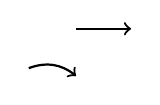
\begin{tikzpicture}\draw[->,thick] (0,0)--(.7,0);\draw[->,thick] (-.6,-.5) to[bend left] (0,-.6);\end{tikzpicture}}
\margin{399}
\margin{271}
\margin{399}
